\documentclass[utf8]{frontiers_suppmat} % for all articles
\usepackage{url,hyperref,lineno,microtype}
\usepackage[onehalfspacing]{setspace}
\usepackage{cleveref}
\usepackage{graphicx}
\usepackage{physics}
\usepackage{siunitx}
\usepackage{interval}
\intervalconfig{soft open fences}
\usepackage{xr}
\externaldocument{manuscript}


\renewcommand{\d}{\mathrm{d}}
\renewcommand{\k}{\mathrm{K}}
\newcommand{\ca}{\mathrm{Ca}}
\newcommand{\na}{\mathrm{Na}}
\newcommand{\leak}{\mathrm{L}}
\newcommand{\dstar}{d^\star}
\newcommand{\gstar}{g^\star}
\newcommand{\gbar}{\bar g}
\newcommand{\delt}{\Delta t}
\newcommand{\taus}{\tau_s}
\newcommand{\dn}{\delta_n}
\newcommand{\taud}{\tau_d}

\graphicspath{{../figures}}

% Leave a blank line between paragraphs instead of using \\

\begin{document}
\onecolumn
\firstpage{1}

\title[Supplementary Material]{{\helveticaitalic{Supplementary Material}}}


\maketitle

\section{Model equations and parameters}
The asymptotic function for the calcium conductance $m_{\infty}$ is given by
\begin{equation}
	m_{\infty}(v) = \frac{1}{2}\left(1+\tanh{\left((v-v_{A})/v_{B}\right)}\right).
\end{equation}
The voltage and potassium nullclines, \(v_{\infty}(v)\) and \(w_{\infty}(v)\), are
\begin{align}
	v_{\infty}(v) & = \frac{-g_{l}(v-v_{l}) - g_{ca}m_{\infty}(v)(v-v_{ca}) + I - \bar g s(v-v_{s})}{g_{k}(v-v_{k})},
	\\
	w_{\infty}(v) & = \frac{1}{2}\left(1+\tanh{\left((v-v_{C})/v_{D}\right)}\right).
\end{align}
Model parameters were adapted from~\cite{bose2011} and are given in \cref{tab:pars}:
\begin{table}[h]
	\caption{Default parameters for coupled Morris-Lecar model.~\label{tab:pars}}
	\centering
	\begin{tabular}{ll}
		Parameter                      & value                 \\
		\hline
		                               &                       \\
		$g_{\leak}$                    & $0.15$ \si{mS/cm^2}   \\
		$g_{\ca}$                      & $0.3$ \si{mS/cm^2}    \\
		$g_{\k}$                       & $0.6$ \si{mS/cm^2}    \\
		$v_{\leak}$                    & $-50$ \si{mV}         \\
		$v_{\ca}$                      & $100$ \si{mV}         \\
		$v_{\k}$                       & $-70$ \si{mV}         \\
		$v_{A}$                        & $1$ \si{mV}           \\
		$v_{B}$                        & $14.5$ \si{mV}        \\
		$v_{C}$                        & $4$ \si{mV}           \\
		$v_{D}$                        & $15$ \si{mV}          \\
		$I$                            & $3.8$ \si{\mu A/cm^2} \\
		$\tau_w$                       & $100$ \si{ms}         \\
		$\tau_a$                       & $1000$ \si{ms}        \\
		$\tau_b$                       & $100$ \si{ms}         \\
		$\tau_\kappa$                  & $100$ \si{ms}         \\
		$v_{\theta}$                   & $0$ \si{mV}           \\
		$v_{s}$                        & $-80$ \si{mV}         \\
		$T$                            & $376$ \si{ms}         \\
		$T_{a}$                        & $49$ \si{ms}          \\
		$T_{s}$                        & $327$ \si{ms}         \\
		$g^{\star}$                    & $0.0068$ \si{mS/cm^2} \\
		$g_{bif}$                      & $0.0038$ \si{mS/cm^2} \\
		$\bar g_{s}$                   & $0.584$ \si{mS/cm^2}  \\
		$\lambda:=\exp(-T_{a}/\tau_b)$ & $0.612$               \\
		$\rho:=\exp(-T_{s}/\tau_a)$    & $0.721$               \\
	\end{tabular}
\end{table}


\section{Computing bifurcation diagram numerically}\label{appendix2}
The bifurcation diagram of stable $n-n$ solutions of the two-cell network in \cref{fig:bif-diagram} is obtained numerically as follows:
We initialise the coupling strength at parameter values associated with one type of $n-n$ solution, that is we choose the values $\bar g = 0.35, 0.4, 0.5, 0.52, 0.56$ for the $1-1$, $2-2$, $3-3$, $4-4$, and $5-5$ solutions respectively.
For each $\bar g$ the system is then numerically integrated sufficiently long for any transients to fully subside.
We then identify one period of the solution by finding the first return of the depression variable $d_{1}$.
That is, we choose some value $d_{k}$ at a spike time $t_{k}$, and by iterating from spike to spike find some subsequent value $d_{k+1}$ at spike time such that $|d_{k+1}-d_{k}|<\epsilon$.
If a periodic solution of type $n-n$ is found in such way, $\bar g$ is step-wise increased/decreased, and the above algorithm is repeated.
Otherwise, the set of all previously found solutions and the corresponding values $\bar g$ are returned.

\section{Numerical validation of constant ISI assumption}
\label{sec:tauk}
% TODO Double-check that you've addressed all of the reviewers concerns here.
% TODO Write caption
To study the effect of the synaptic time constant $\tau_\kappa$ on consecutive $ISI$s of the active cell we consider a single cell that is inhibited by an exponentially decaying synaptic conductance $g$:
\begin{align}
	\label{eq:dotv}
	\dot v & = f(v, w) - g(v - v_{s}), \\
	\label{eq:dotw}
	\dot w & =h(v, w),                 \\
	\label{eq:dotg}
	\dot g & = -g/\tau_{\kappa},
\end{align}
where functions $f$ and $h$ come from \cref{eq:f,eq:h}.
We assume that the cell is released and fires its first spike at time $t=0$.
We therefore initialise $v$ at the firing threshold $v_{\theta}$, $w$ at its nullcline, and
the $g$ at the release conductance $g^{\star}$, respectively:
\begin{align}
	v(0) & = v_{\theta}, \\
	w(0) & = v(0),       \\
	g(0) & = g^{\star}.
\end{align}
We vary $\tau_{\kappa}$ and integrate the system numerically to record consecutive $ISI$s.

\Cref{fig:tauk-vs-ISI} shows the curves for the first ($ISI_{1}$), second ($ISI_{2}$), and third ($ISI_{3}$) inter-spike-intervals for values $\tau_{\kappa} \in \interval[open left]{0}{800}$.
These results suggest that for $\tau_\kappa \leq 100$ we have $ISI_i \approx T$, that is, inhibition $g$ decays sufficiently fast for its effect on the spiking period to be negligible.
For $\tau_\kappa > 100$ the first $ISI_{1}$ becomes increasingly longer with $\tau_{\kappa}$, moreover the effect of the inhibition propagates to the subsequent $ISI_{2}$ and $ISI_{3}$, suggesting that for a too slow synaptic time constant the assumption $ISI \approx T$ is not suitable.

\begin{figure}[h!]
	\centering
	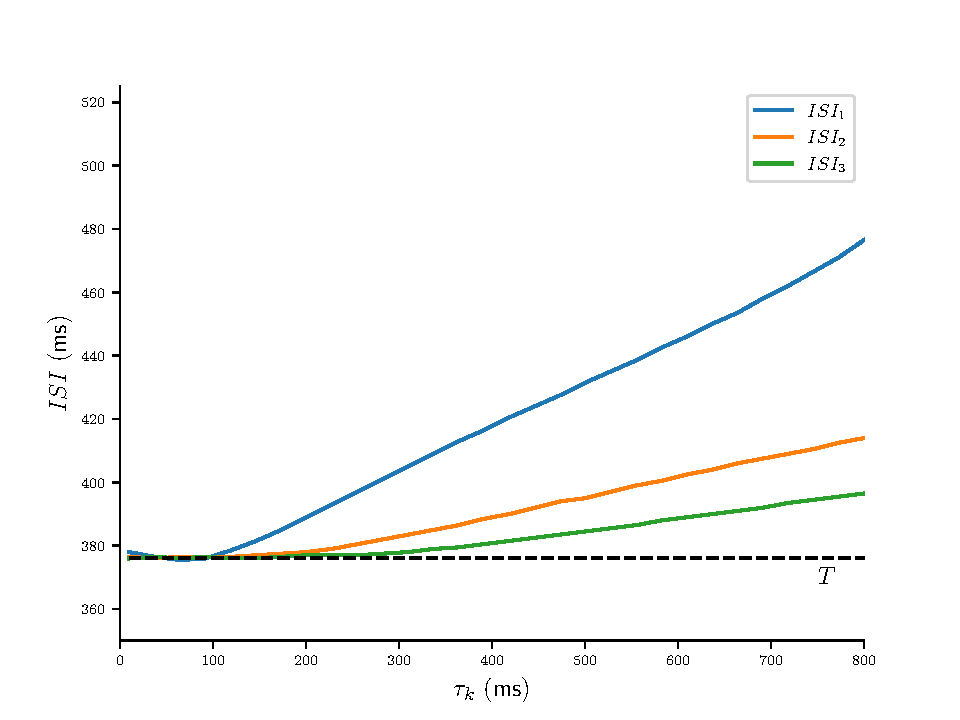
\includegraphics[width=0.8\textwidth]{tauk-vs-ISI}
	\caption{Voltage traces of both cells of numerically stable solutions for increasing
		values of the coupling strength $\gbar$ (increasing top to
		bottom).~\label{fig:tauk-vs-ISI}}
\end{figure}

% TODO
% **Note of caution**: Our ICs might be inaccurate for very large $\tau_\kappa$ , since then $w(0) \approx w_\infty(g^\star)$ will be likely violated.

% \section{Irregular solutions}
% Even

\bibliographystyle{frontiersinHLTH&FPHY} % for Health, Physics and Mathematics articles
\bibliography{bibliography.bib}

\end{document}

%%% Local Variables:
%%% mode: latex
%%% TeX-master: t
%%% End:
